\appendix
\label{sec:appendix}

\section{Triplets generation heuristics}
\label{sec:triplet-generation-heuristics}

\subsection{Triplets selection}

For each anchor data point, we fix a target distance, and a delta percentage.
We can in this way find a first data point which distance to the anchor data point is close to the fixed target distance.

Then, we can find a second data point which distance to the anchor data point is close to the fixed target distance \textbf{plus} a percentage of this target distance, defined by delta. We have to be careful not to propose the same data point here (especially working with small values).

The proposed triplet is the concatenation of these three data points. In the following, for simplicity, we will call these 3 data points respectively the anchor, the positive and the negative, even if the proposed negative can actually be the real positive (hard triplet).

This selection process is shown in \autoref{fig:triplet_generation}. 

\begin{figure}[]
    \centering
    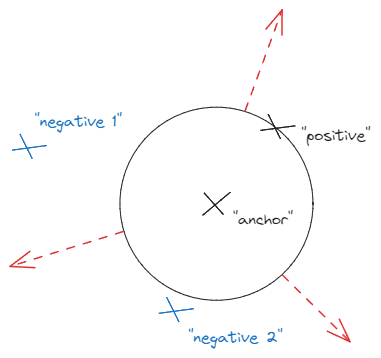
\includegraphics[width=0.4\columnwidth]{images/triplet_generation.png}
    \caption{Triplet selection process. An "anchor" point is selected, and a "positive" point is found at a fixed target distance. A "negative" point is then found at a distance defined by the target distance plus a delta percentage. How far is the negative point matters a lot. If negative 1 is chosen, the triplet will likely be easy to label, but will not bring a lot of value to the model. If negative 2 is chosen, the triplet will likely be hard to label (and thus skipped), but will bring a lot of value to the model.}
    \label{fig:triplet_generation}
\end{figure}

We initially used target distances uniformly distributed between 0.001 and 0.05, and delta uniformly distributed between 0.1 and 0.5.

These hyperparameters must be tuned according to the dataset. Iterative visual inspections were conducted to ensure that the triplets generated were relevant according to the properties defined in \autoref{sec:triplet-generation}.

\subsection{Triplets filtering}

Once our triplets are selected, we have to filter some triplets that do not bring enough value, or that will be too hard for the user to label.

\begin{enumerate}
    \item  Concatenation of the triplets found for each pair of parameters can lead to duplicate triplets -> Duplicated triplets are discarded.
    \item  It turns out that triplets with the same anchor and positive points share really similar negative point -> Duplicated (anchor, positive) triplets are discarded.
    \item Working with small target distances and deltas can lead to undesirable behaviours -> Triplets where the distance from the anchor to the positive $0$ are discarded. Triplets where the distance from the anchor to the positive is greater than the distance from the anchor to the negative are discarded.
    \item Sometimes, the positive and the negative data points turn out to be pretty similar -> Triplets where the relative distance from the positive to the negative is greater than a percentage of the distance from the anchor to the positive are discarded.
\end{enumerate}

All these filters aim at reducing as much as possible the amount of triplets that won't be labeled by the user.